\documentclass[../../main.tex]{subfiles}
\usepackage{listings}
\usepackage{tablefootnote}
\begin{document}
\chapter{Multi-Track and Non-Linear Synthesis}
\label{ch:multi_track}

Human movement is a symphony of coordinated actions, where each part of the body plays a distinct role, yet all work together in harmony to create a seamless expression of intent. The essence of this coordination lies in the ability to perform multiple actions simultaneously or in carefully timed sequences, with each movement contributing to the larger tapestry of physical expression.

Traditional approaches to animating human movement often oversimplify this complexity, reducing it to linear bone rotations. In contrast, multi-track control offers a more nuanced perspective by recognizing the layered, interconnected nature of gestures and postures, reflecting the true complexity of human movement. In the previous chapter, we discussed the creation of an avatar and the generation of signs using AZee's constraints. This chapter shifts focus to the time structure of the animation working from the AZee \emph{Synced Score} structure. As discussed in section \ref{ch:background_work:sign_language_descriptions:azee} of chapter \ref{ch:background_work}, the AZee Synced Score is a recursive representation of the AZee description, where each block represents the motion that holds the specification of the sign. The previous synthesizer for AZee descriptions used a \emph{flattened} Animated Score to generate the animation (explained in section \ref{ch:background_work:sign_language_synthesis:3d_techniques:sign_language_synthesis_systems:azee_based:low_level_synthesizer_for_azee:animated_score} of chapter~\ref{ch:background_work}). However, this flattening process loses the multi-track information present in the original AZee description. In this work, we aim to preserve the dynamics of the individual blocks in the AZee Synced Score and synthesize them directly on a multi-track timeline. By preserving the dynamics of individual animation blocks, this method enhances reusability, accuracy, and flexibility in the synthesis process.

The content of this chapter is structured as follows. Section~\ref{ch:multi_track:score_to_timeline} introduces the process of converting an AZee Synced Score into a multi-track timeline, outlining the benefits of this representation. Section~\ref{ch:multi_track:azee_nl} explores the implications of non-linear synthesis within the AZee framework, particularly how block evaluation order influences the final animation. In Section~\ref{ch:multi_track:resolve_conflicts}, we discuss strategies for resolving conflicts between overlapping animation blocks to ensure smooth and accurate motion. Section~\ref{ch:multi_track:second_pass} details the second-pass evaluation process, focusing on cyclic block sets, transpath blocks, and hold blocks to refine the animation. Section~\ref{ch:multi_track:preanim_blocks} addresses the integration of pre-animated blocks into the multi-track timeline, emphasizing both the benefits and challenges of this approach. Finally, Section~\ref{ch:multi_track:implem_results} presents the implementation and results of our multi-track and non-linear synthesis approach, demonstrating improvements in animation quality, flexibility, and procedural generation.

\section{AZee Synced Score to Multi-Track Timeline}
\label{ch:multi_track:score_to_timeline}

To directly create a multi-track timeline from an AZee Synced Score structure, we parse the Synced Score recursively until we arrive at the lowest (constraint) level of description. We then put these blocks on the timeline based on their sync rules. The algorithm~\ref{alg:azee_timeline} shows how the AZee Synced Score is converted into a multi-track timeline.

\begin{algorithm}
    \caption{AZee Recursion Algorithm (Simplified)}
    \label{alg:azee_timeline}
    \begin{algorithmic}[1]
        \Function{CreateBlocks}{name, score, parent\_name, parent\_score, dynamic\_points}
            \If {parent\_score is not None}
                \State name $\gets$ name + "." + parent\_name
                \State \Call{UpdateSyncRules}{parent\_score, name}
            \EndIf
            
            \State \Call{UpdateBlockTimings}{name, score, parent\_name, parent\_score}
            \If {score.dynamic\_point}
                \State dynamic\_points.append(score.dynamic\_point)
            \EndIf
            
            \If {shortcut\_action $\gets$ \Call{GetShortcutAction}{score} \textbf{and} UseShortcutActions()}
                \State \Return \Call{CreateShortcutBlock}{name, score, parent\_score}
            \ElsIf {score is a SyncedScore}
                \For {child\_name, child\_score in score.block\_contents}
                    \State \Call{CreateBlocks}{child\_name, child\_score, name, score, dynamic\_points}
                \EndFor
            \Else
                \State \Return \Call{CreateRegularBlock}{name, score, parent\_score}
            \EndIf
            
            \If {parent\_score is not None}
                \State \Call{UpdateParentTimings}{parent\_name, name}
            \EndIf
        \EndFunction
    \end{algorithmic}
\end{algorithm}

The figure~\ref{fig:azee_timeline} shows the generated multi-track timeline for \emph{:armoire}.

\begin{figure}[h]
    \centering
    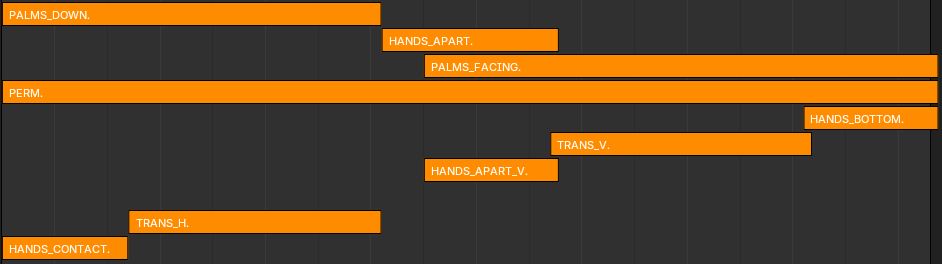
\includegraphics[width=0.6\textwidth]{chapters/multi_track/images/azee_timeline.png}
    \caption{Multi-track timeline generation from an AZee Synced Score.}
    \label{fig:azee_timeline}
\end{figure}

Since we are not flattening the AZee Synced Score, the constraints in the blocks can have dependencies on each other. Also, we have to solve for constraints inside each block to generate an animation. For this, we choose to represent each block's constraints as a \gls{dag}, where the nodes are the constraints and the edges represent the dependencies between them. During evaluation, a topological sort allows us to find the solving order for the constraints. Figure~\ref{fig:constraint_dag_armoire} shows an example of a ConstraintDAG for the block HANDS\_CONTACT for the sign \emph{armoire} (figure \ref{fig:armoire_sign}). A more complex DAG of constraints can be seen in figure~\ref{fig:constraint_dag_tree} for the sign \emph{arbre} (\gls{lsf} tree) (figure \ref{fig:tree_sign}).

\begin{figure}[h]
    \centering
    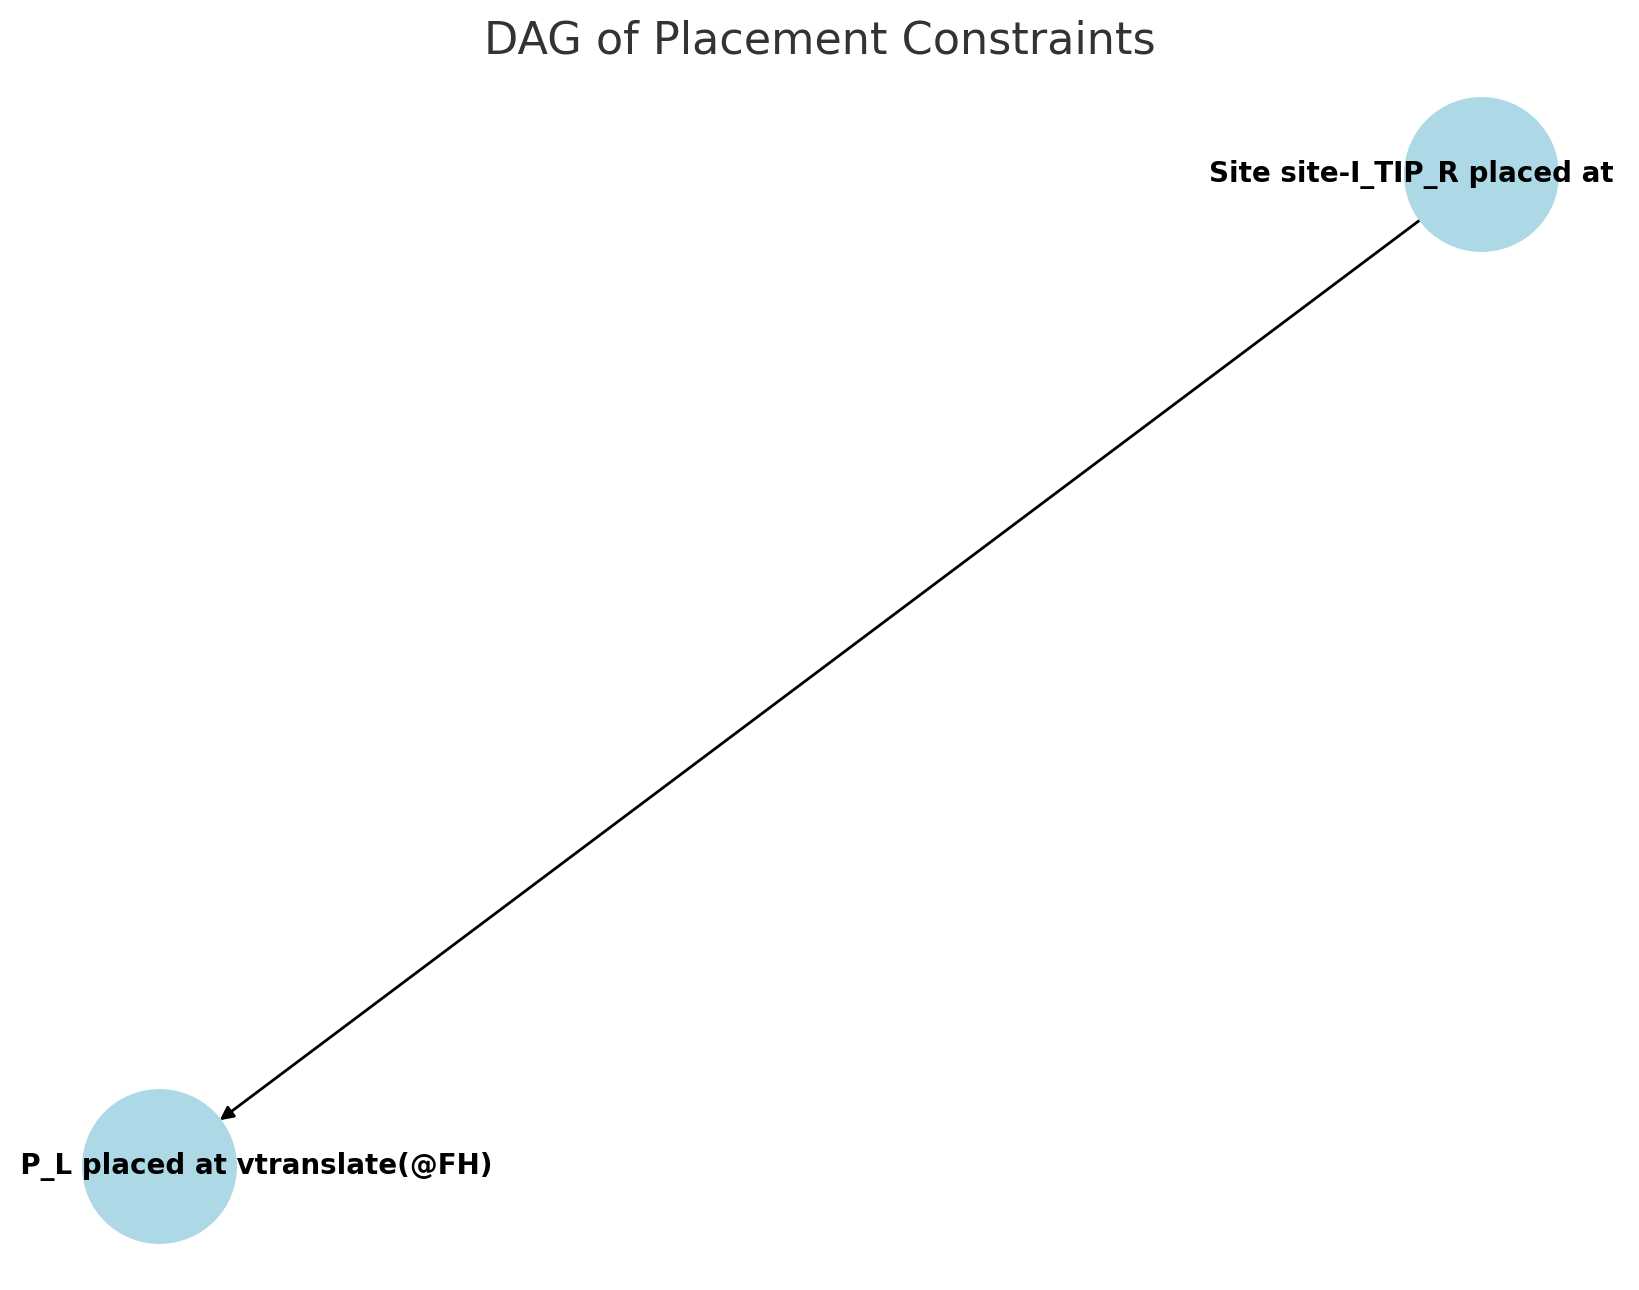
\includegraphics[width=0.6\textwidth]{chapters/multi_track/images/constraint_dag_cupboard.png}
    \caption{ConstraintDAG for a single block discourse for the block HANDS\_CONTACT from the sign \emph{armoire}}
    \label{fig:constraint_dag_armoire}
\end{figure}

\begin{figure}[h]
    \centering
    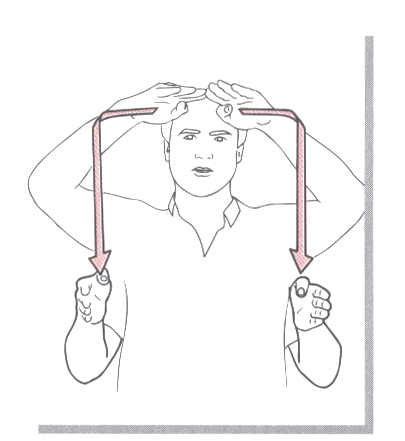
\includegraphics[width=0.5\textwidth]{chapters/multi_track/images/cupboard.jpg}
    \caption{Sign \emph{armoire}~\cite{moody97} with AZee blocks}
    \label{fig:armoire_sign}
\end{figure}

\begin{figure}[h]
    \centering
    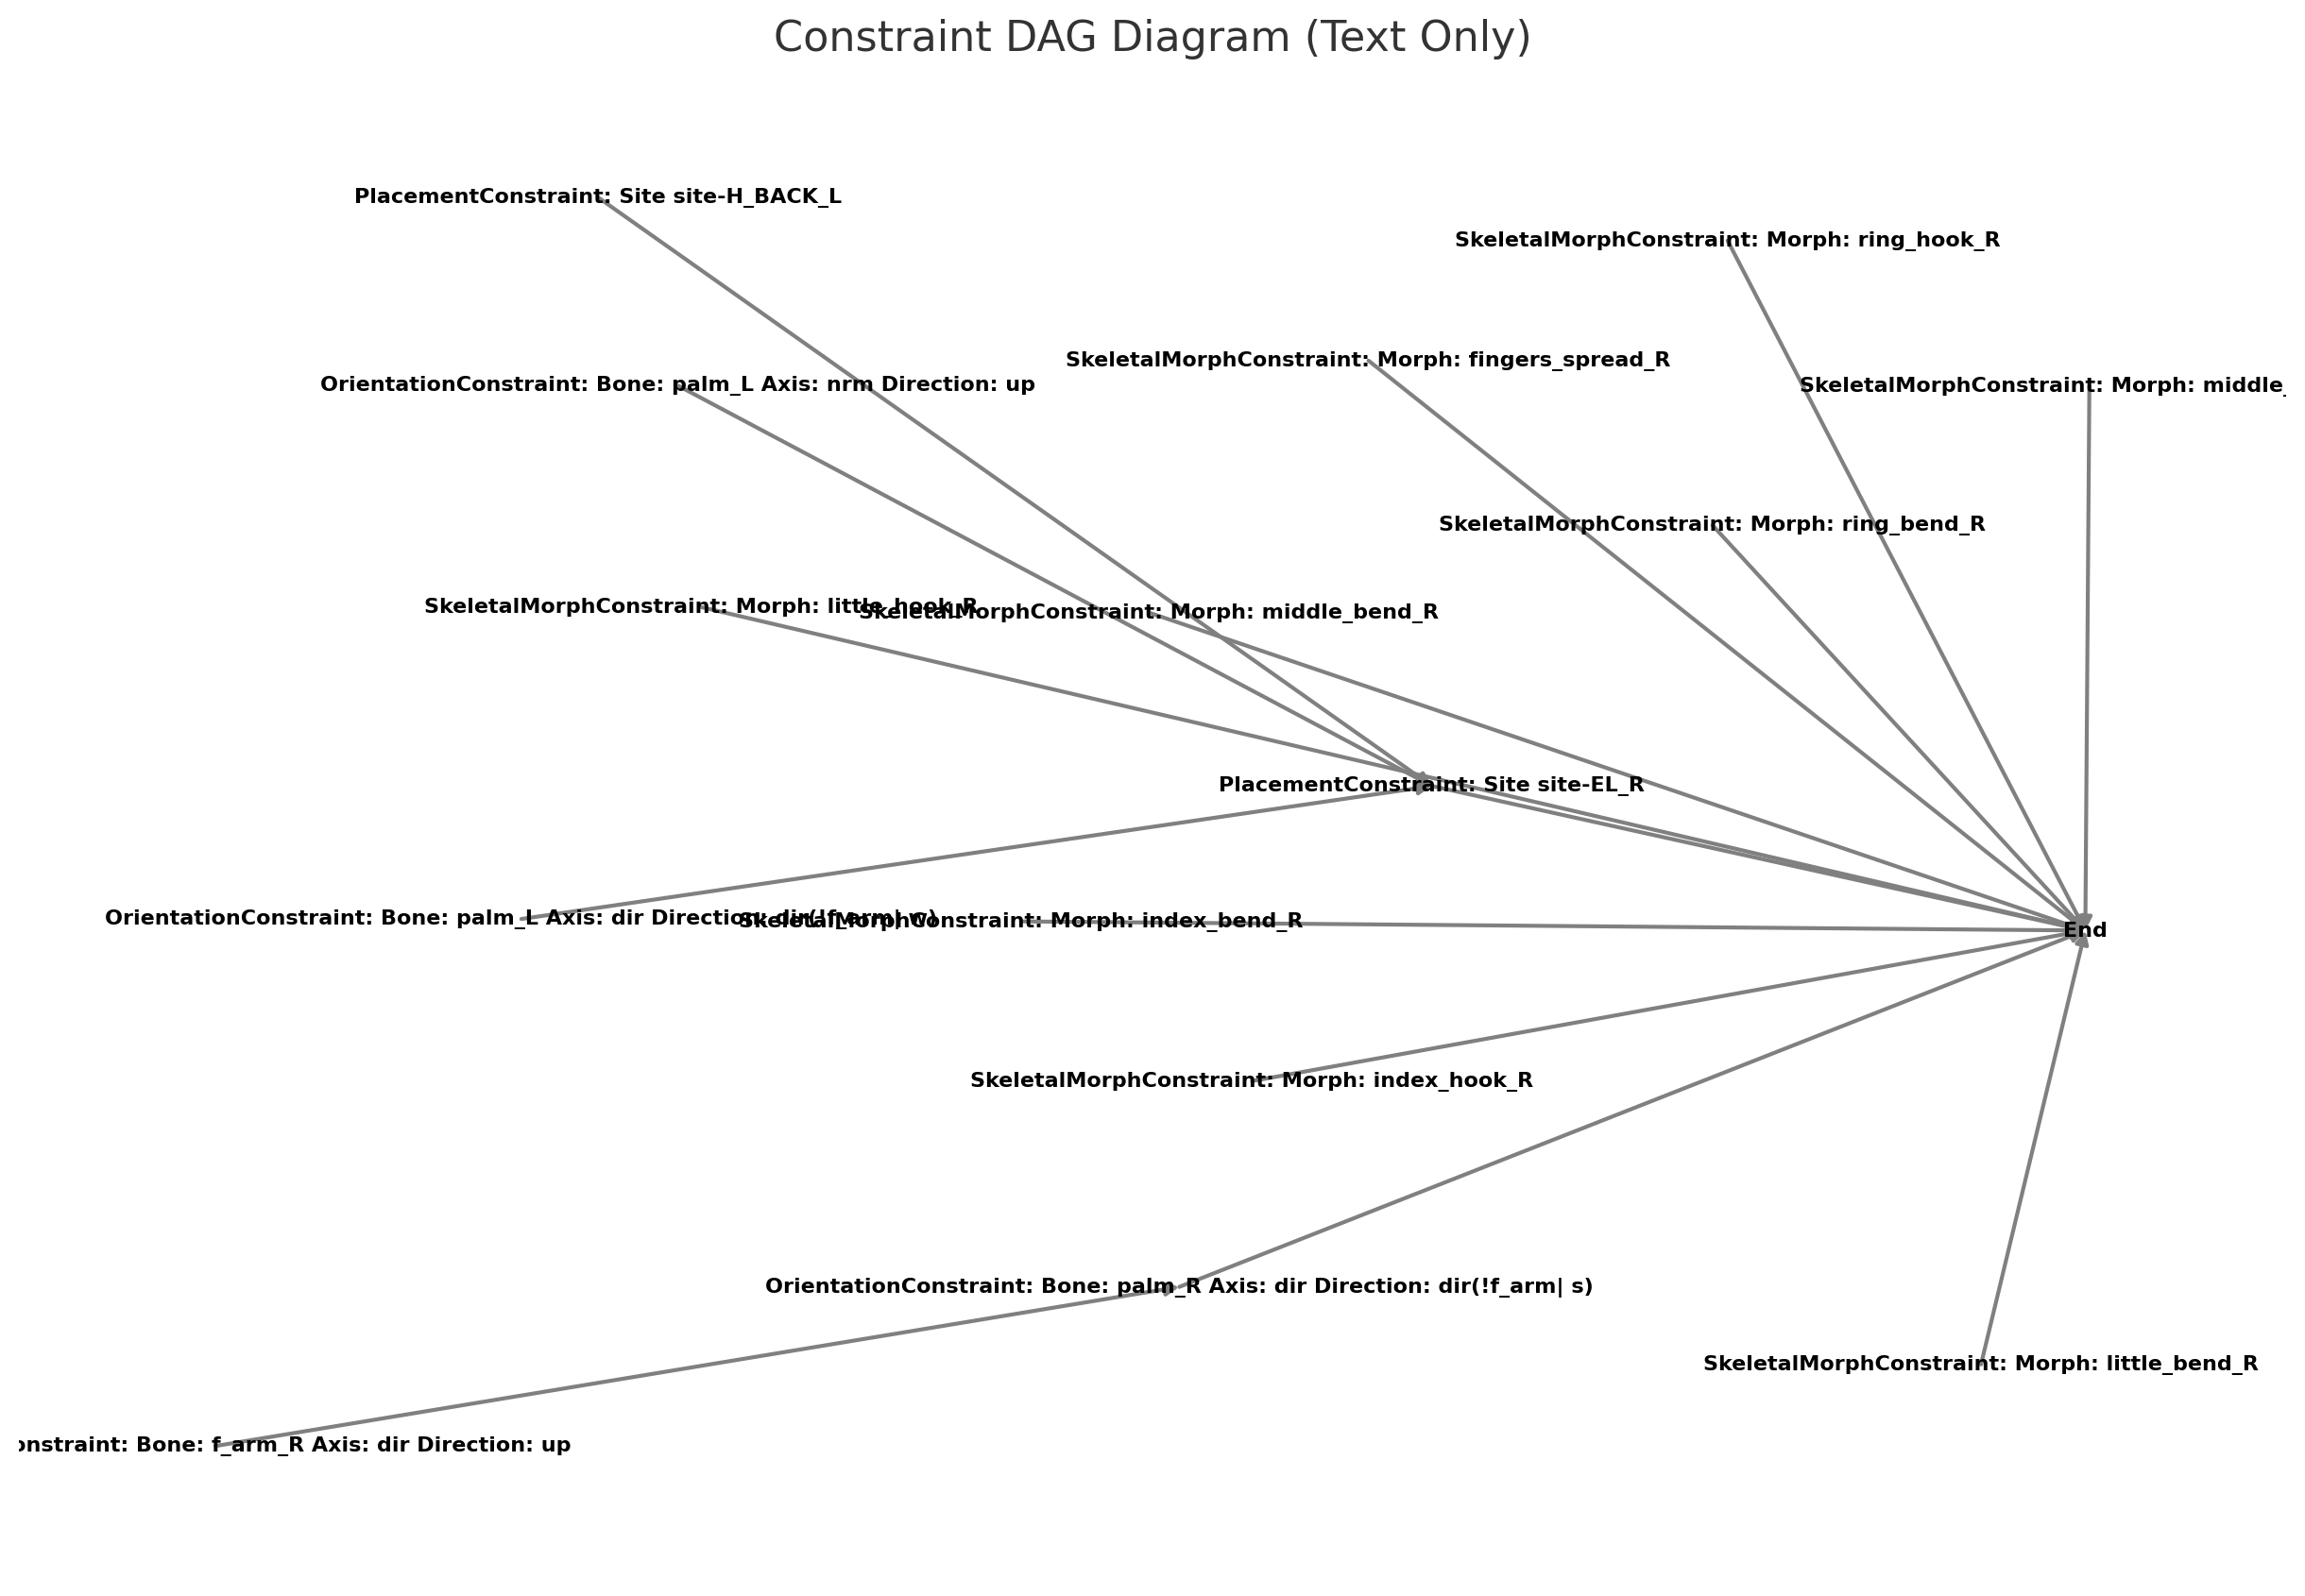
\includegraphics[width=0.8\textwidth]{chapters/multi_track/images/constraint_dag.png}
    \caption{ConstraintDAG for a single block discourse for the sign \emph{arbre}.}
    \label{fig:constraint_dag_tree}
\end{figure}

\begin{figure}[h]
    \centering
    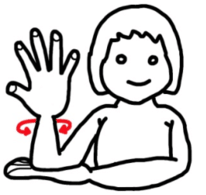
\includegraphics[width=0.5\textwidth]{chapters/multi_track/images/tree.png}
    \caption{Sign \emph{arbre}~\cite{boutetetal}}
    \label{fig:tree_sign}
\end{figure}

\section{AZee and Non-Linearity}
\label{ch:multi_track:azee_nl}

\begin{figure}[H]
    \centering
    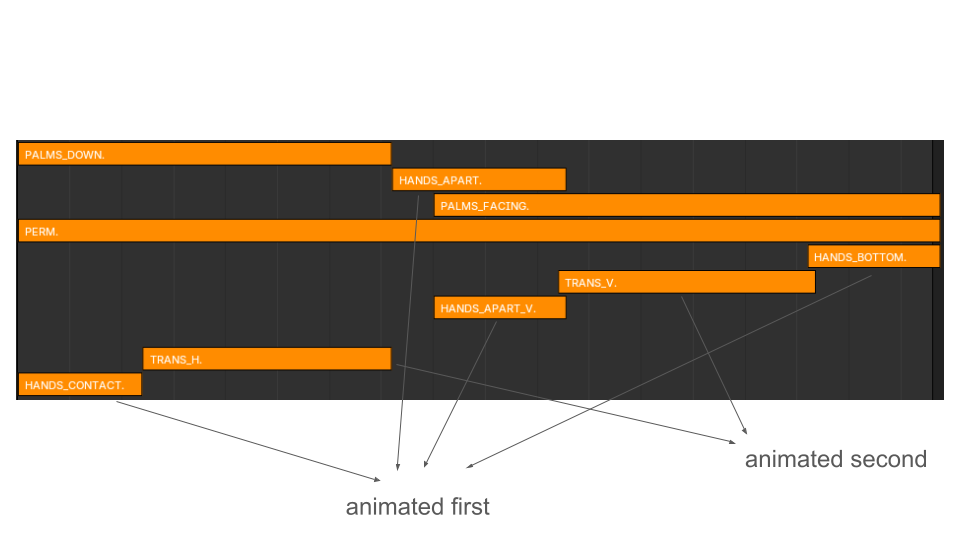
\includegraphics[width=0.6\textwidth]{chapters/multi_track/images/example_azee_non_linear.png}
    \caption{Example of non-linear synthesis in AZee.}
    \label{fig:example_azee_non_linear}
\end{figure}

Just like the order of the constraints inside the blocks, the order of synthesis of the blocks in the multi-track timeline is crucial as well in order to avoid conflicts and ensure the correct execution of constraints. Due to these dependencies, an action that happens later in the timeline might be synthesized first. As a result, the synthesis process becomes non-linear.

For example, the \emph{transpath} block TRANS\_H in the sign \emph{armoire} is evaluated after the block such as HANDS\_APART for the sign \emph{armoire}. This is because this constraint requires resolution of both initial and final positions for the hand IK chain. Figure~\ref{fig:example_azee_non_linear} shows non-linear synthesis for the sign \emph{armoire}.

\section{Resolving Block Conflicts}
\label{ch:multi_track:resolve_conflicts}

Since a pair of blocks in the multi-track timeline can have constraints that affect the same body parts, conflicts can arise. For example, both blocks PALMS\_DOWN and HANDS\_CONTACT affect both the palm bones. Such conflicts need to be resolved to ensure the correct execution of the constraints. To resolve these conflicts, we follow the following rules:

\subsection{Rule 1: Timely Evaluation}
\label{ch:multi_track:resolve_conflicts:rule1}

\textbf{Problem:} Overlapping blocks with different start times. \\

\textbf{Example:} Let's consider the timeline in figure~\ref{fig:azee_timeline} for the sign \emph{armoire} (figure~\ref{fig:armoire_sign}). Here, blocks PALMS\_DOWN (palms facing down) and HANDS\_APART (hands being apart) overlap (affect the same bones, i.e., the hand chains at the same time).  \\

\textbf{Solution:} Evaluate blocks chronologically to maintain a logical sequence, i.e., the block that starts first is evaluated first. Thus, the block, PALMS\_DOWN, is evaluated first before the block HANDS\_APART.  \\

\subsection{Rule 2: Constraint Precedence}
\label{ch:multi_track:resolve_conflicts:rule2}

\textbf{Problem:} Some constraints might affect the same body part but have different priorities. \\

\textbf{Example:} For the same timeline in figure~\ref{fig:azee_timeline}, the block HANDS\_CONTACT contains two constraints, a placement of hands contacting each other at a small distance from the forehead, and the orientation of the wrist along the forearm. \\

\textbf{Solution:} Follow the constraint precedence order: \emph{placement}, \emph{transpaths}, \emph{lookat}, \emph{trill}, \emph{orientation}, and then \emph{morph}. The block HANDS\_CONTACT optimizes the posture for placements first, then the orientations of the wrists. \\

Non-overlapping blocks can be evaluated in parallel since they won't disrupt the posture. For example, blocks PERM and HANDS\_CONTACT are a non-overlapping block set in the sign \emph{armoire}.

\section{Second Pass}
\label{ch:multi_track:second_pass}

A second pass is done on the timeline to synthesize cyclic block sets, transpath, and hold blocks.

\subsection{Cyclic Block Set}
\label{ch:multi_track:second_pass:cyclic_blocks}

Cyclic block sets, as the name suggests, are blocks with cyclic dependencies on each other. Figure~\ref{fig:cyclic_blocks} shows a cyclic block set for HANDS\_CONTACT and PALMS\_DOWN. This problem could arise if blocks affect a common hierarchy of the skeleton (any changes in the parent will affect the child even if the blocks don't affect that part of the skeleton), or even if they affect each other directly. To deal with such sets, the blocks are evaluated again in a second pass by optimizing for a \emph{cumulative flattened loss}, i.e., collecting the loss of all constraints of the block set for the frame and optimizing them together through iterations.

\begin{figure}[h]
    \centering
    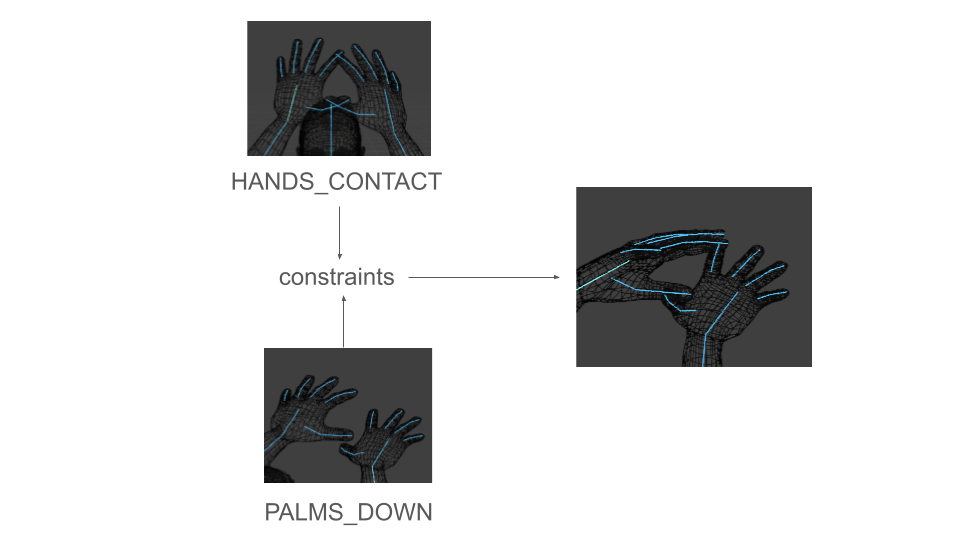
\includegraphics[width=0.8\textwidth]{chapters/multi_track/images/cyclic_blocks.png}
    \caption{Cyclic block set for PALMS\_DOWN and HANDS\_CONTACT.}
    \label{fig:cyclic_blocks}
\end{figure}

\subsubsection{Baking Cyclic Blocks}
\label{ch:multi_track:second_pass:cyclic_blocks:baking_cyclic_blocks}

Even though the constraints are optimized together, each individual block in the cyclic block set is baked separately to preserve the multi-track structure of the discourse. This is done by collecting the \emph{change in motion curves} of each block and applying them separately to the skeleton after the optimization step.

\subsection{Transpath Blocks}
\label{ch:multi_track:second_pass:transpath_blocks}

\begin{figure}[h]
    \centering
    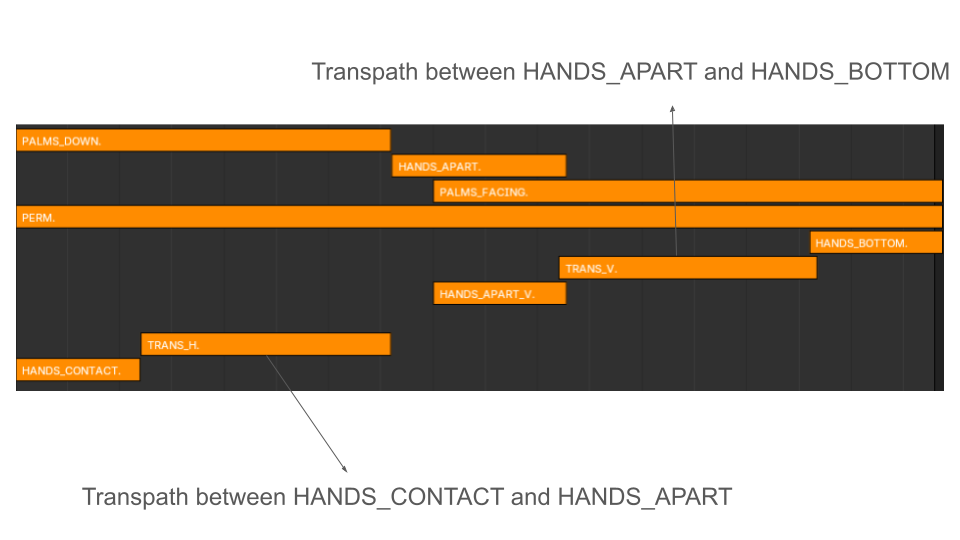
\includegraphics[width=0.6\textwidth]{chapters/multi_track/images/transpath_blocks.png}
    \caption{Transpath blocks in \emph{armoire}}
    \label{fig:transpath_blocks}
\end{figure}

Transpath blocks are blocks that contain one or more transpath constraints. As discussed earlier in section~\ref{ch:background_work:sign_language_descriptions:azee:low_level} of chapter~\ref{ch:background_work}, a transpath constraint moves a body site along a path. It acts as a transition (interpolation) block but with a controlled path for a particular body site for its preceding and following block. Figure~\ref{fig:transpath_blocks} shows an example of transpath blocks for the sign \emph{armoire}. Just like cyclic block sets, transpath blocks are evaluated in a second pass.

Transpath blocks are baked by evaluating the transpath constraint for each frame and applying the change in motion curve of the body site with respect to the preceding and the succeeding block. These motion curves are then baked as a new block.

\subsection{Hold Blocks}
\label{ch:multi_track:second_pass:hold_blocks}

\begin{figure}[H]
    \centering
    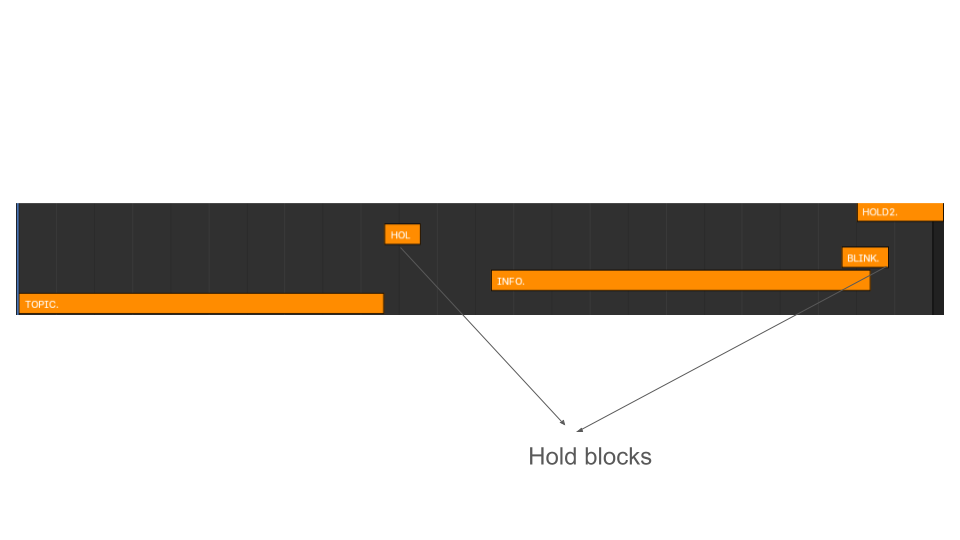
\includegraphics[width=0.6\textwidth]{chapters/multi_track/images/hold_blocks.png}
    \caption{Hold blocks for the rule \emph{:info-about(:topic, :info)}}
    \label{fig:hold_blocks}
\end{figure}

Hold blocks are blocks that hold another block for a certain duration. Figure~\ref{fig:hold_blocks} shows an example of hold blocks for the rule \emph{:info-about(:topic, :info)}. Hold blocks are also evaluated in the second pass since they hold another block (which has to be evaluated in the 1st pass).

Hold blocks are baked by extending the end of the motion curves of the block being held. This extension is not applied to the last values of motion curves but to a set of values that are calculated by the hold block itself.

\section{Pre-animated blocks}
\label{ch:multi_track:preanim_blocks}

\begin{figure}[H]
    \centering
    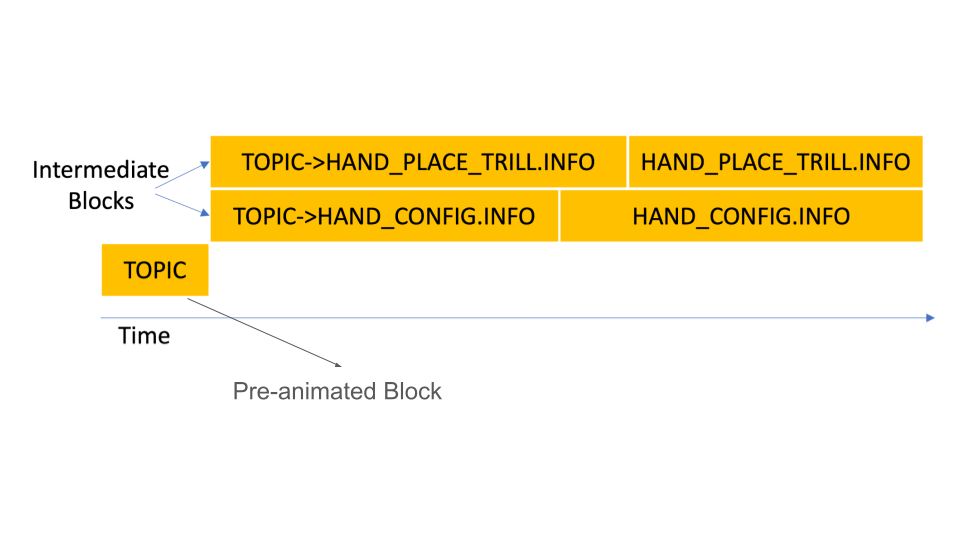
\includegraphics[width=0.6\textwidth]{chapters/multi_track/images/preanim_blocks.png}
    \caption{Pre-animated blocks in the multi-track timeline.}
    \label{fig:preanim_blocks}
\end{figure}

% describe the blocks here

The timeline can also contain pre-animated blocks. These blocks are blocks that contain pre-animated motion data. The pre-animated blocks are evaluated and baked first since they are independent of other blocks (figure~\ref{fig:preanim_blocks}) and should not influence the other blocks in the timeline.

\section{Implementation and Results}
\label{ch:multi_track:implem_results}

The multi-track timeline is implemented in blender's \gls{nle}. Each AZee Score, when animated, generates a blender action which is put on the \gls{nle} as a strip with a duration specified by the AZee \emph{sync rules}. The following table~\ref{tab:azee_to_blender} shows some AZee expressions with their timelines and synthesized animations.

\begin{table}[H]
    \centering
    \begin{tabular}{|c|p{4.5cm}|p{2cm}|}
        \hline
        \textbf{AZee expression} & \textbf{Timeline} & \textbf{Animation} \\
        \hline
        \texttt{:armoire} & 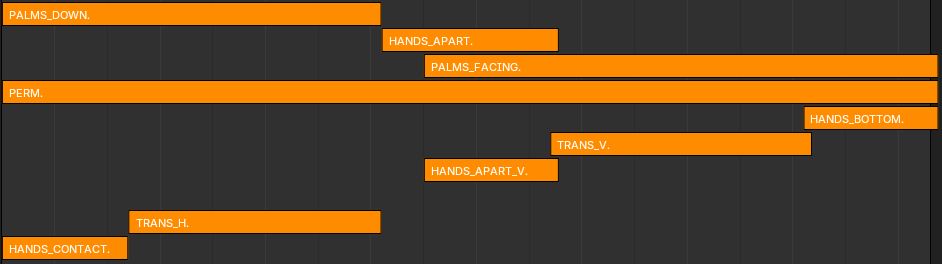
\includegraphics[width=\linewidth]{chapters/multi_track/images/azee_timeline.png} & Video ~\tablefootnote{\url{https://github.com/Paritosh97/phd/raw/master/supplementary_material/ch4armoire.mp4}} \\
        \hline
        \texttt{:bien} & 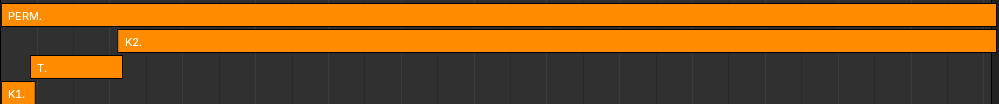
\includegraphics[width=\linewidth]{chapters/multi_track/images/bien_timeline.png} & Video 2~\tablefootnote{\url{https://github.com/Paritosh97/phd/raw/master/supplementary_material/ch4bien.mp4}} \\
        \hline
        \parbox{5cm}{
          \raggedright
          \texttt{:info-about} \newline
          \makebox[1cm]{} \texttt{'topic} \newline
          \makebox[1cm]{} \texttt{:personne} \newline
          \makebox[1cm]{} \texttt{'info} \newline
          \makebox[1cm]{} \texttt{:info-about} \newline
          \makebox[2cm]{} \texttt{'topic} \newline
          \makebox[2cm]{} \texttt{:âge} \newline
          \makebox[2cm]{} \texttt{'info} \newline
          \makebox[2cm]{} \texttt{:tens-units} \newline
          \makebox[3cm]{} \texttt{'tens} \newline
          \makebox[3cm]{} \texttt{.nb-5} \newline
          \makebox[3cm]{} \texttt{'units} \newline
          \makebox[3cm]{} \texttt{.nb-2}
        } & 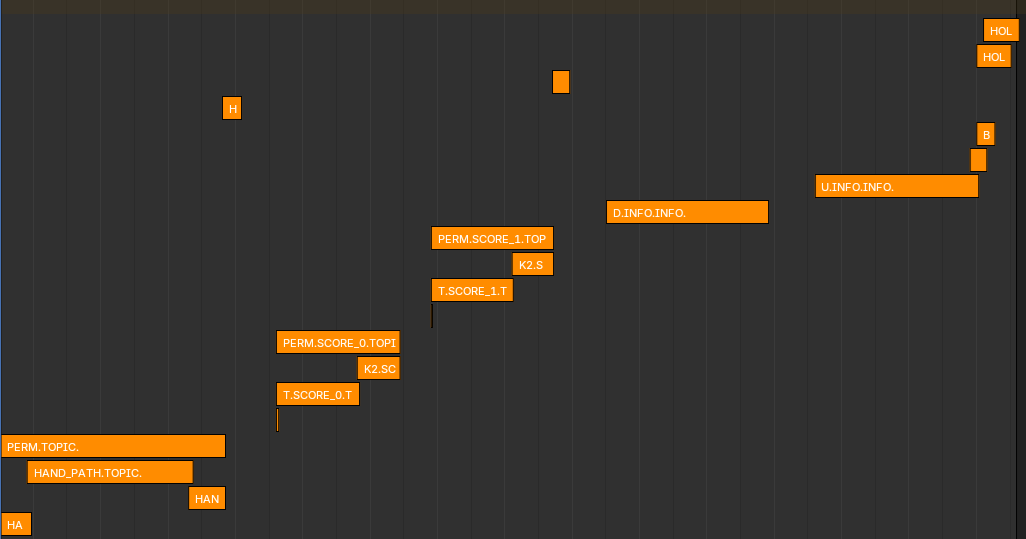
\includegraphics[width=\linewidth]{chapters/multi_track/images/result_ch4_persone_age_52_timeline.png} & Video 3~\tablefootnote{\url{https://github.com/Paritosh97/phd/raw/master/supplementary_material/ch4person52.mp4}} \\
        \hline
    \end{tabular}
    \caption{Multi-track timeline and synthesized animations for some AZee expressions}
    \label{tab:azee_to_blender}
\end{table}

We observe that each of the movement on the avatar's skeleton is based on the track created by AZee Synced Score. For more complex utterances, the importance of this is more obvious compared to simple stitching of glosses which most of the earlier models proposed. This also enables us to use hybrid constructs in AZee such as \emph{dynamic points} (a point changing its location over time) where motion inside parallel blocks affect each other. This can be seen for the sign \emph{mercredi} (Wednesday in \gls{lsf}) (figure~\ref{fig:dynpoint_example}).

\begin{figure}[h]
    \centering
    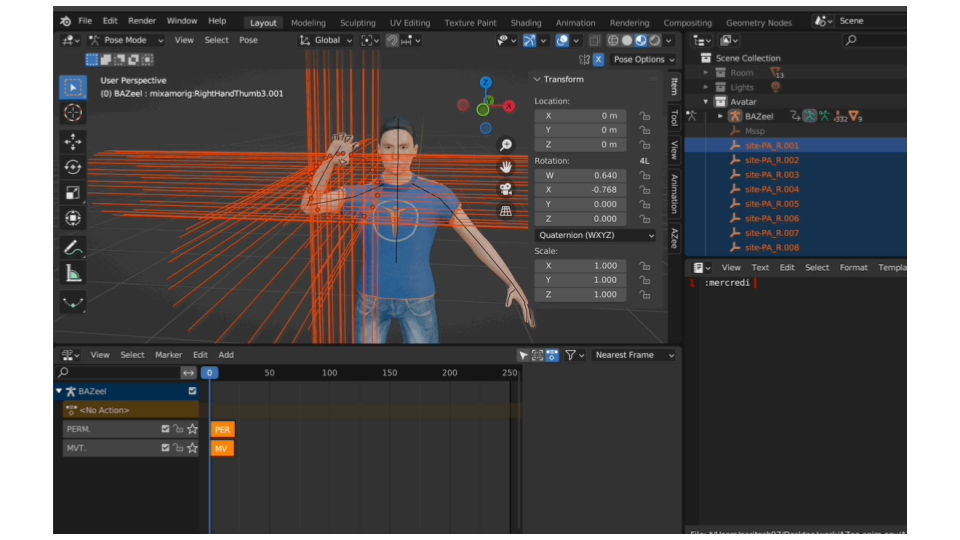
\includegraphics[width=0.6\textwidth]{chapters/multi_track/images/dynpoint_example.png}
    \caption{Example of a dynamic point in the multi-track timeline for \emph{mercredi}}
    \label{fig:dynpoint_example}
\end{figure}

\section{Conclusion}
\label{ch:multi_track:conclusion}

The multi-track timeline approach to \gls{sl} synthesis offers several advantages over the existing methods. Preserving the multi-track information and dynamics present in the AZee description provides us the stepping stones to integrate pre-animated motion data which was not possible with the previous low-level AZee synthesizer. The non-linear synthesis allows for the correct execution order of blocks and avoids conflicts. However, there are future avenues open for this research such as:

\begin{itemize}
    \item \textbf{Parallelism in block generation} Our system cannot generate multiple independent blocks at the same time in parallel. This could greatly speedup the time for animation
    \item \textbf{Smartly keyframing} An effort was made to "smartly" keyframe postures to increase synthesis speed, however it didn't work when the AZee Scores contained complex structures such as \emph{dynamic points} (created as a centripetal Catmull–Rom spline) in the linguistic discourse. Thus, we optimize the constraints for every frame of the block which is not the most efficient way to animate the block.
\end{itemize}

\end{document}
